\adparagraph{Borda Count}
Aside from SF in the SFD measure, and Adjusted nDCG, BC was the best performing method.
\begin{figure}[H]
	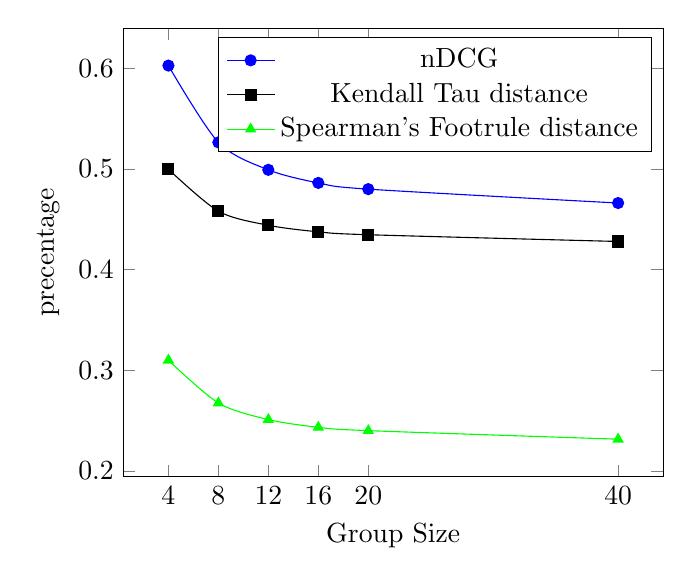
\begin{tikzpicture}
	\begin{axis}[
	xlabel=Group Size,
	ylabel=precentage,
	xtick = {4,8,12,16,20,40}]
	\addplot[smooth,mark=*,blue] plot coordinates {
		(4,0.6028)
		(8,0.5265)
		(12,0.4992)
		(16,0.4862)
		(20,0.48)
		(40,0.4662)
	};
	\addlegendentry{nDCG}
	
		\addplot[smooth,color=black,mark=square*] plot coordinates {
		(4,0.4998)
		(8,0.4581)
		(12,0.4441)
		(16,0.4376)
		(20,0.4347)
		(40,0.428)
	};
	\addlegendentry{Kendall Tau distance}
	
		\addplot[smooth,color=green,mark=triangle*] plot coordinates {
		(4,0.31)
		(8,0.2675)
		(12,0.251)
		(16,0.2433)
		(20,0.24)
		(40,0.2315)
	};
	\addlegendentry{Spearman's Footrule distance}
	
	\end{axis}
	\end{tikzpicture}
	\caption{Results for Borda Count}\label{fig:ndcganalysis}
\end{figure}

\begin{table}[H]
\centering
\label{my-label}
\begin{tabular}{|l|lllll|}\hline
     & 4 to 8 & 8 to 12 & 12 to 16 & 16 to 20 & 20 to 40 \\\hline
nDCG & 12.66  & 5.19    & 2.6      & 1.28     & 2.88     \\
KTD  & 8.34   & 3.06    & 1.46     & 0.66     & 1.54     \\
SFD  & 13.71  & 6.17    & 3.07     & 1.36     & 3.54     \\\hline
\end{tabular}
\caption{Percentage decrease between the groups for Borda Count}
\end{table}